\section{Resultados}
\label{sec:resultados}

\subsection{O sinal de teste}

O sinal usado é o do enunciado, gerado com a semente indicada para que o resultado seja reprodutível. Ele é a soma de quatro coisas: o canal útil em $30$~kHz com amplitude $1$ e uma pequena modulação de amplitude, o canal adjacente em $200$~kHz com amplitude $8$, o interferente em $450$~kHz com amplitude $6$ e um ruído fraco de amplitude $0{,}01$.

A Figura~\ref{fig:sinal} mostra esse sinal de duas maneiras. Em cima, no tempo: as partes real (I) e imaginária (Q) somadas dão uma forma de onda embaralhada, com picos passando de $15$, e é impossível enxergar o canal útil no meio disso — ele tem amplitude $1$ contra vizinhos de amplitude $8$ e $6$. Embaixo, no espectro, cada componente aparece separada na sua frequência, e o desenho fica imediatamente legível.

\begin{figure}[htb]
\centering
\caption{Sinal recebido em banda base: no tempo (acima) e no espectro (abaixo), com $0$~dB tomado no canal útil.}
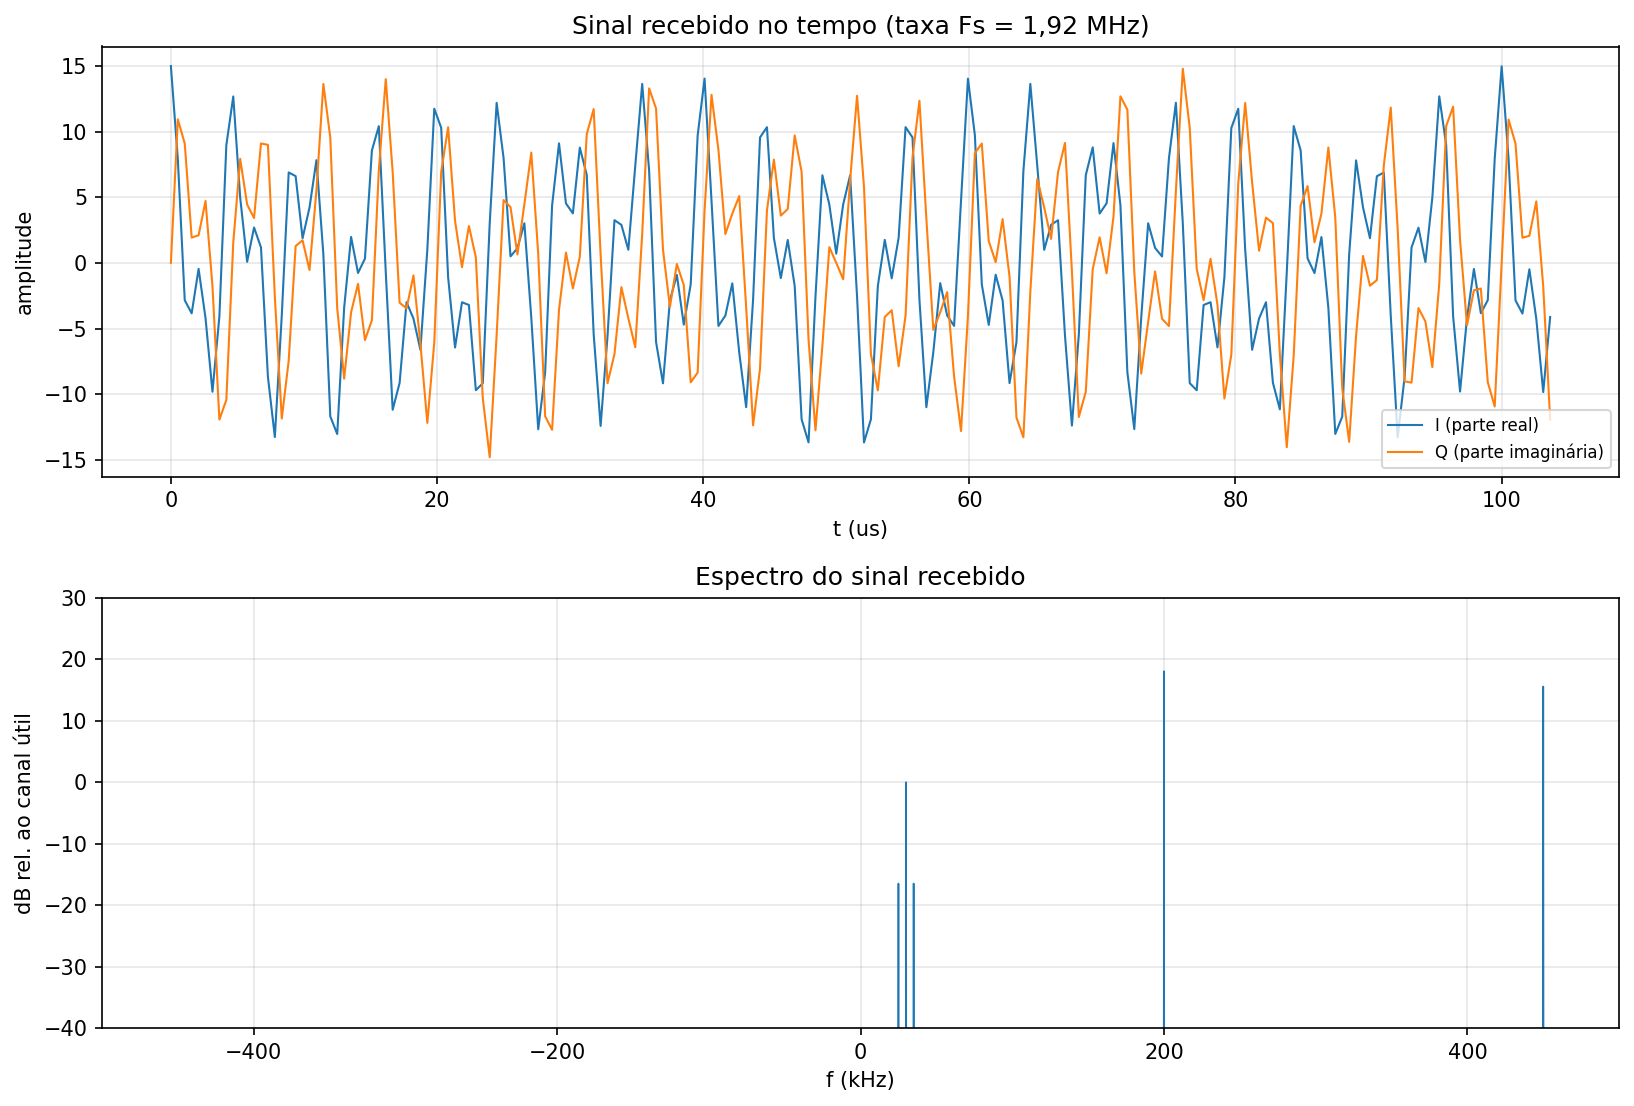
\includegraphics[width=\linewidth]{Imagens/fig01_sinal_recebido.png}
\label{fig:sinal}
\fonte{Autoria própria.}
\end{figure}

Vale explicar por que cada raia está onde está, e com aquela altura.

\begin{enumerate}[a)]
\item \textbf{A raia em $30$~kHz, no nível $0$~dB.} É o canal útil. Ela foi escolhida como referência de $0$~dB do gráfico, então todas as outras alturas são lidas em relação a ela. As duas raias menores logo ao lado, em $25$ e $35$~kHz e cerca de $16$~dB abaixo, não são um sinal separado: são as bandas laterais criadas pela modulação de amplitude. Multiplicar a portadora por $(1 + 0{,}3\,\mathrm{sen}(2\pi 5000t))$ produz duas cópias afastadas de $5$~kHz para cada lado, cada uma com amplitude $0{,}15$, o que dá exatamente $20\log_{10}(0{,}15) = -16{,}5$~dB.

\item \textbf{A raia em $200$~kHz, $18{,}1$~dB acima.} É o canal adjacente. A altura vem direto da amplitude que ele tem no sinal: $20\log_{10}(8/1) = 18{,}06$~dB. Ele está em $200$~kHz porque é a posição do canal vizinho depois que o DDC trouxe o canal de interesse para o zero.

\item \textbf{A raia em $450$~kHz, $15{,}6$~dB acima.} É o interferente forte. A altura, de novo, é só a razão de amplitudes: $20\log_{10}(6/1) = 15{,}56$~dB. A frequência não é acidental: $450$~kHz foi escolhida no enunciado justamente porque, ao decimar por $4$, ela cai exatamente em cima do canal útil.

\item \textbf{O piso em torno de $-73$~dB.} É o ruído. Ele não forma raia porque está espalhado por todas as frequências, e não concentrado em uma só.
\end{enumerate}

O ponto que esses números deixam claro é que o filtro não precisa apenas atenuar: ele precisa atenuar o suficiente para vencer a vantagem de $18$ e $15{,}6$~dB com que os interferentes chegam. Foi disso que saiu a atenuação de projeto de $75{,}56$~dB discutida na Seção~\ref{sec:metodologia}.

\subsection{A resposta em frequência do filtro}

A Figura~\ref{fig:resposta} traz os três gráficos pedidos, com as bordas de $100$ e $200$~kHz marcadas por linhas tracejadas nos três painéis.

\begin{figure}[htb]
\centering
\caption{Resposta em frequência do filtro projetado: magnitude, fase e atraso de grupo.}
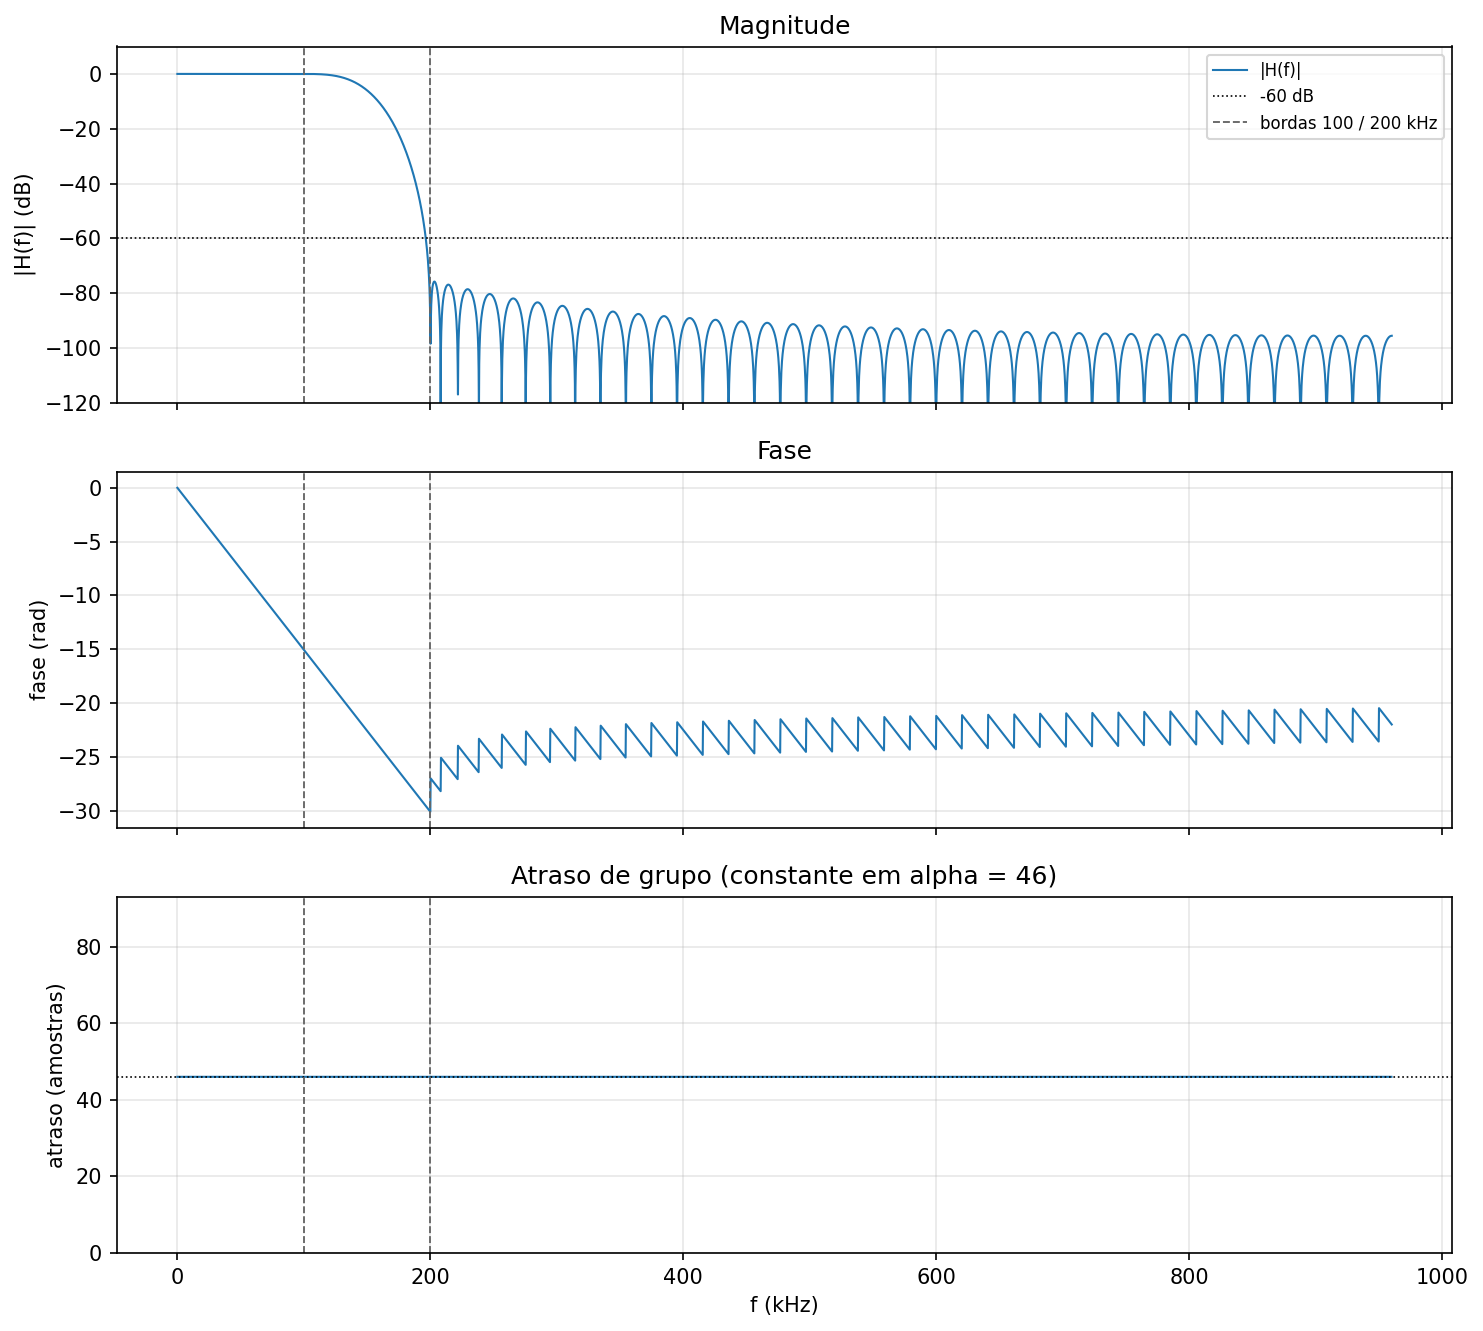
\includegraphics[width=0.92\linewidth]{Imagens/fig03_resposta_frequencia.png}
\label{fig:resposta}
\fonte{Autoria própria.}
\end{figure}

\textbf{A magnitude} (painel de cima) mostra o comportamento esperado de um passa-baixas: ganho praticamente constante até $100$~kHz, uma descida rápida na faixa de transição e, a partir de $200$~kHz, uma sucessão de lóbulos que nunca sobem acima de $-75$~dB. A linha pontilhada marca os $-60$~dB do enunciado, e dá para ver que a resposta passa bem abaixo dela — a sobra é justamente a atenuação extra que o interferente exigiu.

\textbf{A fase} (painel do meio) é uma reta descendente dentro da faixa de passagem, que é a assinatura da fase linear. Os dentes de serra que aparecem depois de $200$~kHz não são distorção: são apenas os pontos onde a magnitude passa por zero, e nesses pontos a fase salta $\pi$. Como ali o sinal já foi atenuado quase $100$~dB, não há nada de relevante acontecendo naquela região.

\textbf{O atraso de grupo} (painel de baixo) é uma reta horizontal em $46$ amostras, do início ao fim da banda. Essa é a prova visual de que o filtro não distorce a fase: todas as frequências saem atrasadas exatamente do mesmo tanto, $46$ amostras ou $23{,}96$~$\mu$s. A verificação numérica confirma: dentro da faixa de passagem, o mínimo e o máximo do atraso são ambos $46{,}0000$ amostras.

\subsection{Antes e depois do filtro}

A Figura~\ref{fig:antes-depois} mostra o efeito do filtro sobre o sinal de teste, em três recortes.

\begin{figure}[htb]
\centering
\caption{Efeito do filtro: espectro na taxa original, espectro após a decimação e comparação no tempo.}
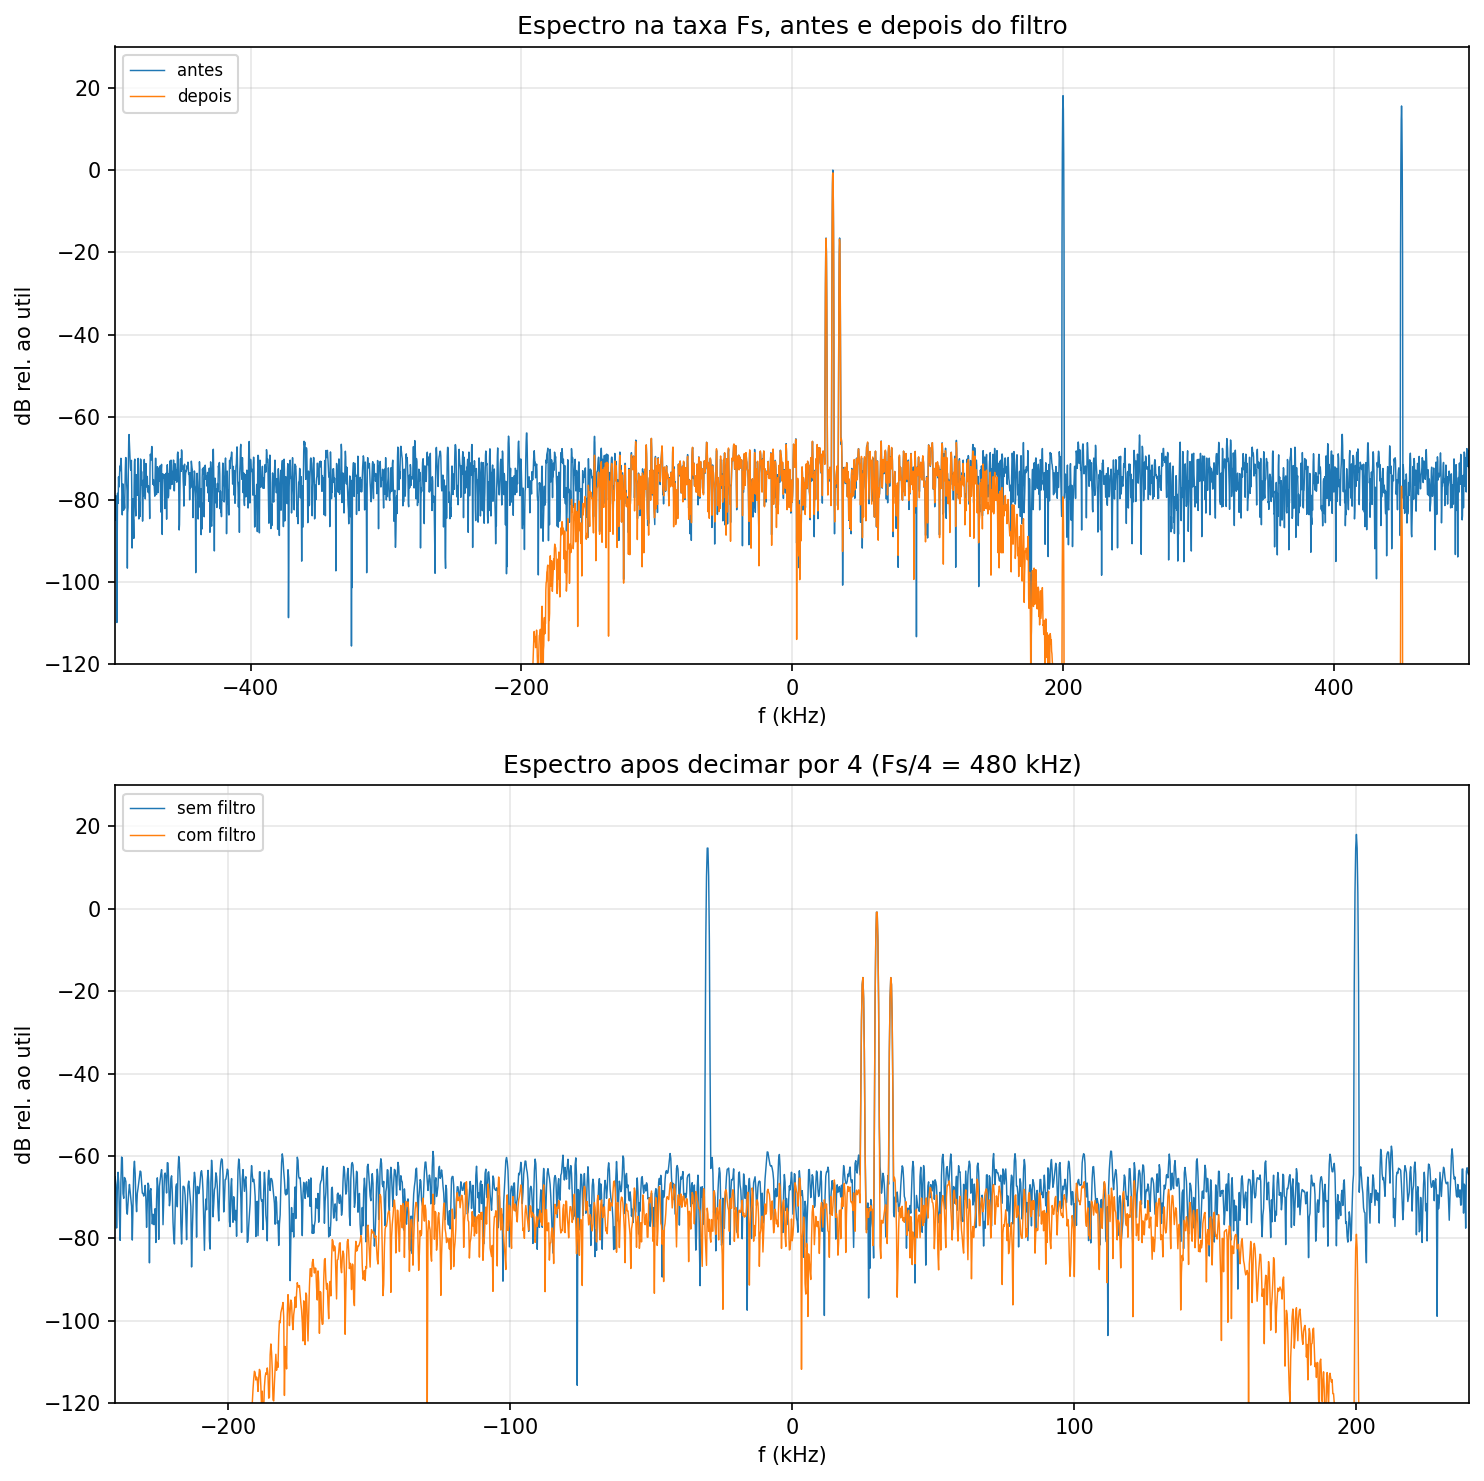
\includegraphics[width=0.92\linewidth]{Imagens/fig04_antes_depois.png}
\label{fig:antes-depois}
\fonte{Autoria própria.}
\end{figure}

No \textbf{painel de cima}, ainda na taxa de $1{,}92$~MHz, a curva ``antes'' tem as três raias descritas na Seção anterior. Na curva ``depois'', as raias de $200$ e $450$~kHz simplesmente somem, e o que resta é o canal útil com suas bandas laterais, exatamente como estavam. Repare também que o piso de ruído cai fora da banda de passagem: o filtro não elimina só os interferentes, ele elimina todo o ruído que estava fora do canal.

O \textbf{painel do meio} é o mais importante do trabalho, porque mostra o problema e a solução lado a lado. A curva ``sem filtro'' é o que aconteceria se decimássemos direto: aparece uma raia em $-30$~kHz que não existia no sinal original — é o interferente de $450$~kHz que dobrou para dentro do canal, exatamente como previsto pela conta $450 - 480 = -30$~kHz. Ela chega com $+15{,}6$~dB, ou seja, quinze decibéis mais forte que o próprio canal que queremos receber. Na curva ``com filtro'' essa raia desaparece por completo, e sobra apenas o canal útil.

O \textbf{painel de baixo} compara no tempo. A curva fina e agitada é a entrada, com os interferentes somados. A curva grossa é a saída depois de filtrar e decimar, e a tracejada é o canal útil original deslocado de $46$ amostras. As duas últimas se sobrepõem quase perfeitamente, o que mostra que o filtro tirou tudo o que sobrava sem estragar o que interessava — só atrasou. O pequeno desencontro nos primeiros microssegundos é o transiente do filtro, que precisa de $M$ amostras para encher a linha de atraso antes de entregar o resultado correto.

\subsection{Decimação polifásica}

Na implementação direta, o filtro é calculado para toda amostra que entra e depois se descarta três de cada quatro resultados. É trabalho jogado fora: cada amostra de saída custa $93 \times 4 = 372$ multiplicações, e três quartos delas produziram números que ninguém usou.

A decomposição polifásica reorganiza a mesma soma. Escrevendo a saída já decimada e separando os coeficientes segundo o resto da divisão por $4$, o filtro se quebra em quatro subfiltros de $24$ coeficientes que já trabalham na taxa baixa. Cada coeficiente passa a ser usado uma única vez por amostra de saída, e o custo cai para $96$ multiplicações — praticamente o fator $4$ da decimação (o valor exato é $3{,}9$ porque foram somados três zeros para fechar quatro ramos iguais).

O ponto importante é que não se trata de uma aproximação. Comparando a saída da implementação direta com a da polifásica, a maior diferença encontrada foi de $1{,}5 \times 10^{-15}$, que é o erro de arredondamento do ponto flutuante. As duas fazem exatamente a mesma conta.

A Figura~\ref{fig:polifasica} confirma no espectro que o resultado da polifásica está correto: dentro do canal útil, marcado pelas linhas tracejadas em $\pm 100$~kHz, não sobrou nem o interferente dobrado nem o canal adjacente.

\begin{figure}[htb]
\centering
\caption{Espectro decimado pela implementação polifásica, comparado com a decimação sem filtro.}
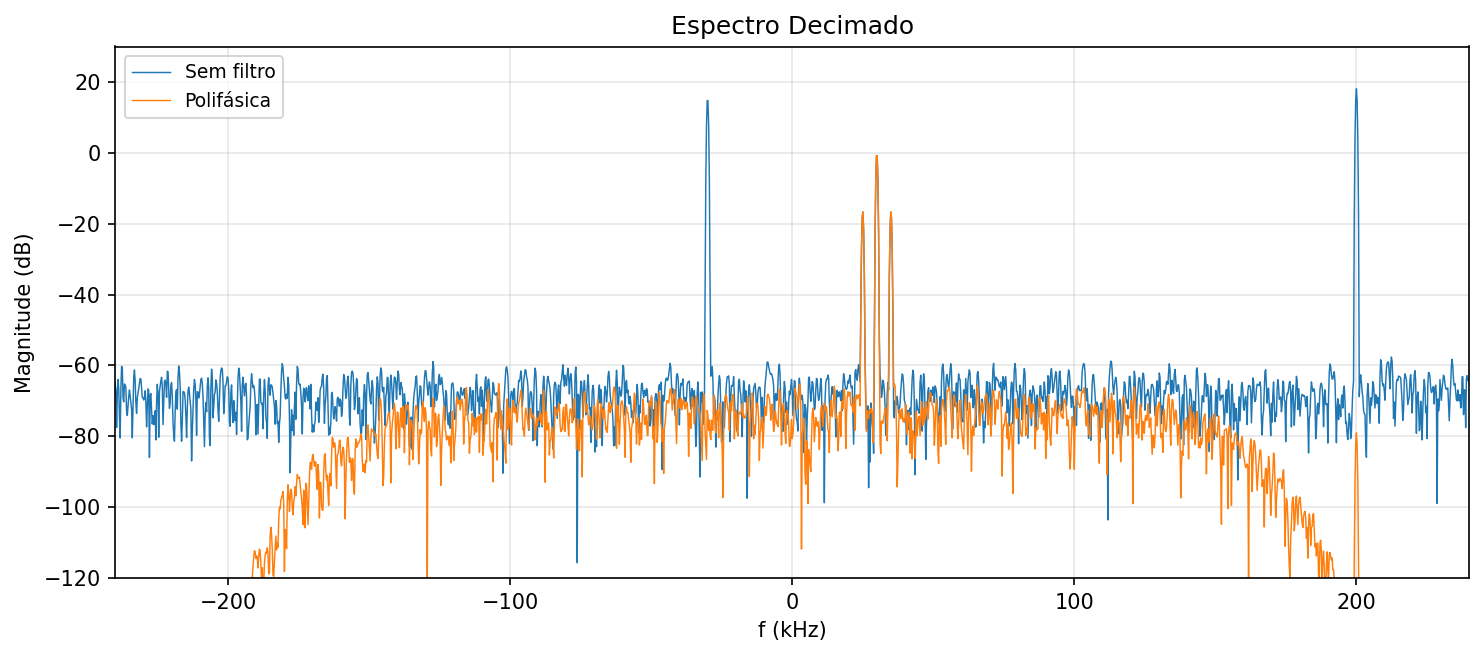
\includegraphics[width=0.92\linewidth]{Imagens/fig05_polifasica.png}
\label{fig:polifasica}
\fonte{Autoria própria.}
\end{figure}

\subsection{Tabela de métricas}

A Tabela~\ref{tab:metricas} reúne as medidas pedidas na Seção 6 do enunciado.

\begin{table}[htb]
\centering
\caption{Métricas obtidas.}
\label{tab:metricas}
\begin{tabular}{p{7.5cm}p{6cm}}
\hline
\textbf{Métrica} & \textbf{Valor obtido} \\
\hline
Número de coeficientes e atraso de grupo & $93$ coeficientes; $46$ amostras ($23{,}96$~$\mu$s) \\
Rejeição medida em $200$~kHz & $97{,}08$~dB \\
Atenuação em $450$~kHz e nível do \textit{aliasing} sobre o canal & $92{,}19$~dB; \textit{alias} em $-71{,}9$~dB abaixo do útil \\
Multiplicações por amostra de saída & $372$ (direta) contra $96$ (polifásica) \\
\hline
\end{tabular}
\fonte{Autoria própria.}
\end{table}

\subsection{Critério de aprovação}

A Tabela~\ref{tab:aprovacao} confronta os valores medidos com os três limites da Seção 7 do enunciado. Todos são atendidos.

\begin{table}[htb]
\centering
\caption{Verificação do critério de aprovação.}
\label{tab:aprovacao}
\begin{tabular}{lccc}
\hline
\textbf{Critério} & \textbf{Exigido} & \textbf{Obtido} & \\
\hline
Rejeição em $200$~kHz & $\ge 60$~dB & $97{,}08$~dB & atende \\
Componente de $450$~kHz dobrada sobre o útil & $\le -60$~dB & $-71{,}9$~dB & atende \\
Ondulação na passagem até $100$~kHz & $\pm 0{,}1$~dB & $0{,}0025$~dB & atende \\
\hline
\end{tabular}
\fonte{Autoria própria.}
\end{table}

Cabe uma observação sobre o segundo valor. A previsão teórica para o \textit{alias} é $15{,}56 - 92{,}19 = -76{,}6$~dB, mas o que se mede no gráfico é $-71{,}9$~dB. A diferença não é erro de projeto: o piso de ruído do sinal de teste está em torno de $-73$~dB, então a raia do interferente já foi empurrada para \emph{abaixo} do ruído e o que se lê naquele ponto do espectro é o próprio ruído. Em outras palavras, o interferente foi eliminado até um nível que o sinal de teste não permite mais enxergar.

\section{Questão conceitual}
\label{sec:conceitual}

\subsection{Por que a fase linear preserva a constelação I/Q}

Quando os coeficientes do filtro são simétricos, ou seja $h[n] = h[M-1-n]$, a resposta em frequência pode ser escrita como

\begin{equation}
H(e^{j\omega}) = A(\omega)\,e^{-j\omega\alpha},
\end{equation}

com $A(\omega)$ real. Toda a dependência da fase com a frequência está naquele expoente, que é uma reta. Derivando, o atraso de grupo dá

\begin{equation}
\tau(\omega) = -\frac{d\theta}{d\omega} = \alpha = 46 \ \mathrm{amostras},
\end{equation}

um valor constante, igual para todas as frequências.

Na prática isso significa que o sinal complexo inteiro sai apenas deslocado no tempo. Nenhuma componente chega antes ou depois das outras, então o símbolo que entrou íntegro sai íntegro, e os pontos da constelação continuam nas mesmas posições. O bloco seguinte só precisa saber que existe um atraso fixo de $46$ amostras, e o sincronizador dá conta disso sozinho.

Se a fase não fosse linear, cada frequência sofreria um atraso diferente. A energia de um símbolo, que deveria chegar concentrada em um instante, se espalharia pelos instantes vizinhos e invadiria os símbolos seguintes — é a interferência entre símbolos. Na constelação, os pontos apareceriam girados e borrados, cada um de um jeito. Como o classificador decide justamente pela geometria desses pontos, ele passaria a confundir uma modulação com outra, e o demodulador erraria a decisão.

\subsection{Por que a polifásica reduz o custo sem perder informação}

A economia vem de perceber que, na filtragem direta seguida de decimação, três de cada quatro resultados são calculados e jogados fora. A polifásica não descobre nenhum atalho matemático: ela apenas separa a soma de modo que só as saídas que serão usadas sejam calculadas.

Partindo da saída já decimada,

\begin{equation}
y[m] = \sum_k h[k]\,x[Dm-k],
\end{equation}

e reescrevendo o índice como $k = qD + p$, com $p$ indo de $0$ a $D-1$:

\begin{equation}
y[m] = \sum_{p=0}^{D-1}\sum_q h[qD+p]\;x[D(m-q)-p]
     = \sum_{p=0}^{D-1}\big(h_p * x_p\big)[m],
\end{equation}

onde $h_p[q] = h[qD+p]$ é o subfiltro $p$ e $x_p[m] = x[Dm-p]$ é a entrada já subamostrada. Cada um dos quatro ramos tem $M/D$ coeficientes e opera na taxa baixa. Somando os ramos, cada coeficiente de $h$ é usado uma única vez por amostra de saída, o que dá o fator $D$ de economia.

Não há perda de informação porque nenhuma parcela foi eliminada da conta: a soma é a mesma, apenas em outra ordem. É por isso que a diferença numérica entre as duas implementações fica no nível do erro de arredondamento.

\subsection{Por que um IIR seria pior aqui}

Para responder a essa parte com número, e não só com argumento, um filtro elíptico foi projetado para as \emph{mesmas} especificações do FIR e os dois foram comparados lado a lado. O elíptico atende com ordem $6$ — três seções de segunda ordem — contra os $93$ coeficientes do FIR. A diferença parece enorme, mas dois problemas anulam essa vantagem.

O primeiro é a fase, e a Figura~\ref{fig:fir-vs-iir} mostra isso de forma direta. Na magnitude (painel superior esquerdo) os dois cumprem a especificação, e o elíptico até desce mais rápido na transição — é a vantagem esperada dele. Mas na fase (painel superior direito) a diferença salta aos olhos: a do FIR é uma reta perfeita, enquanto a do IIR é curva e cheia de quebras. A consequência aparece no atraso de grupo (painéis inferiores): o FIR é uma linha horizontal em $46$ amostras, enquanto o IIR varia de $11{,}90$ a $35{,}75$ amostras dentro da faixa de passagem, ou seja, $23{,}86$ amostras de dispersão — $12{,}42$~$\mu$s.

\begin{figure}[htb]
\centering
\caption{FIR de fase linear contra IIR elíptico projetado para as mesmas especificações.}
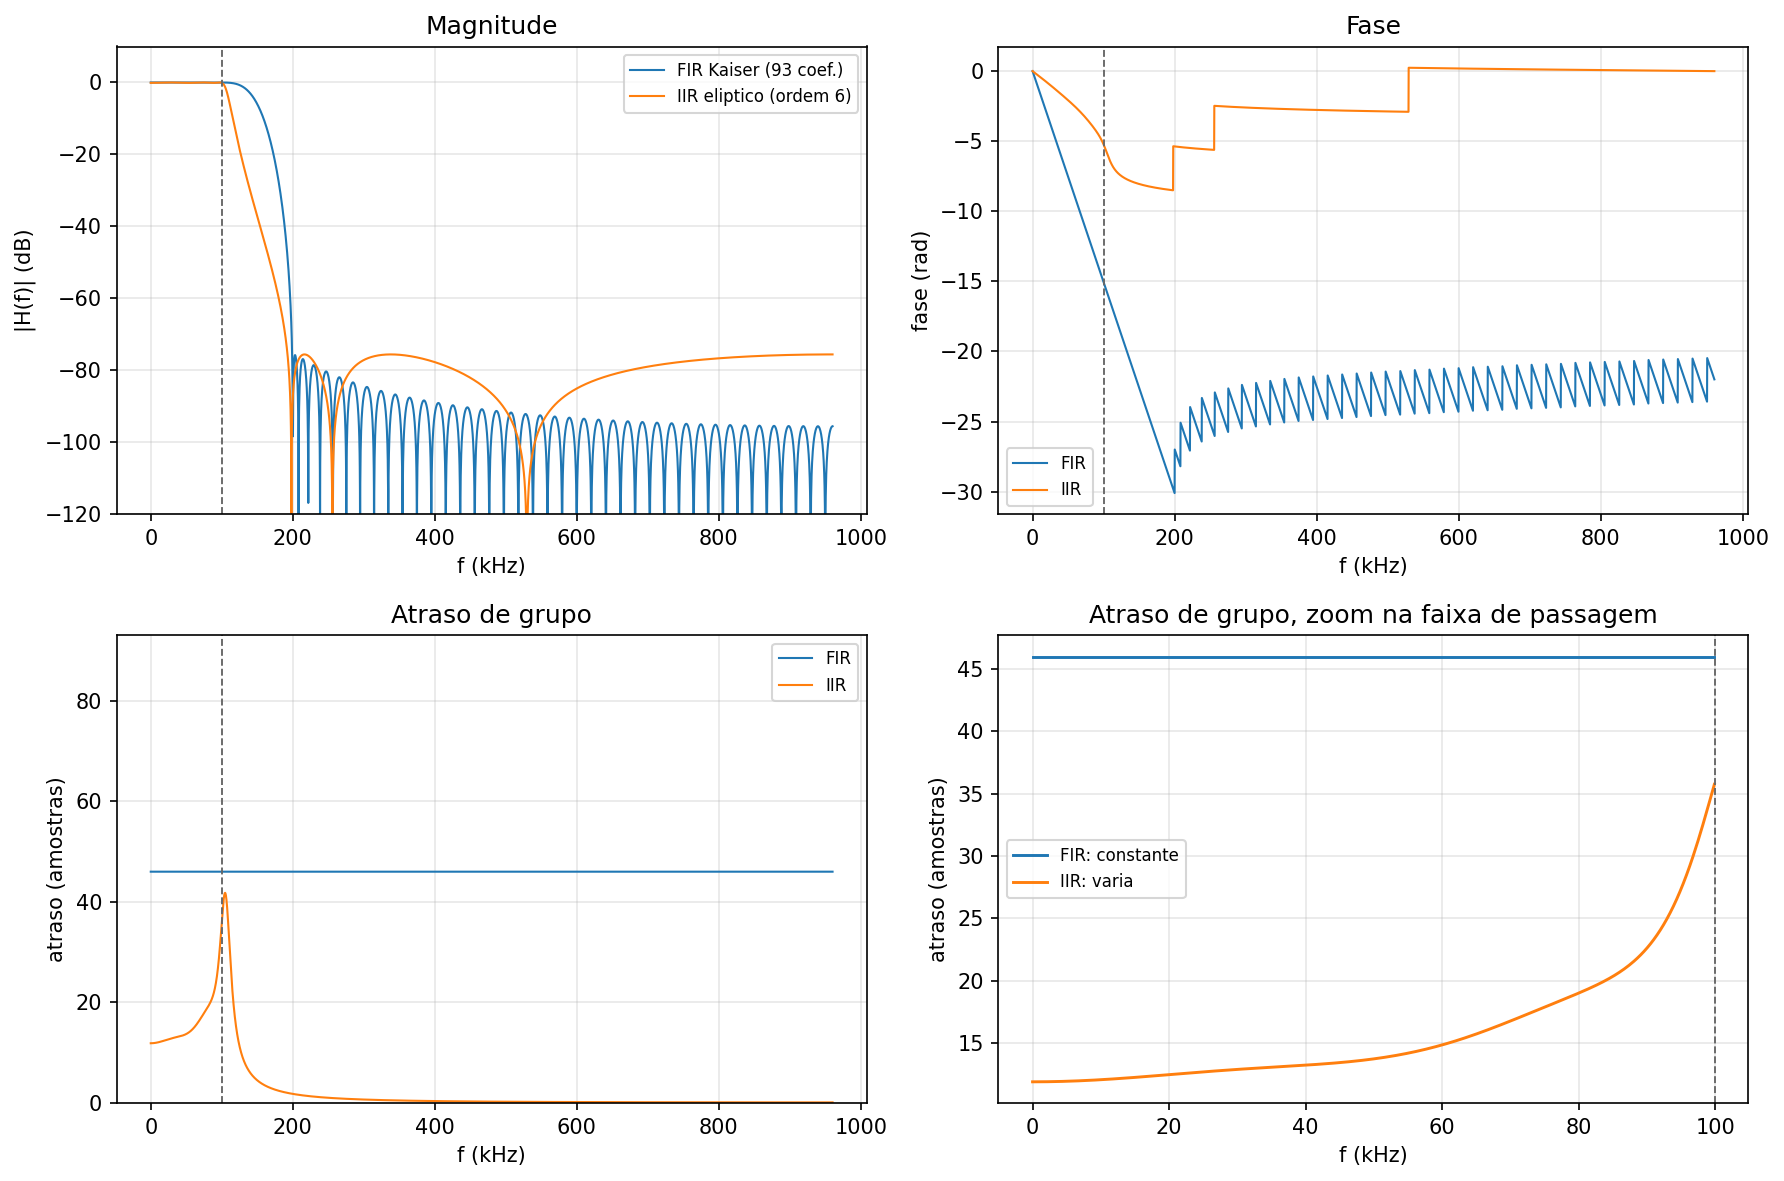
\includegraphics[width=\linewidth]{Imagens/fig06_fir_vs_iir.png}
\label{fig:fir-vs-iir}
\fonte{Autoria própria.}
\end{figure}

O zoom no canto inferior direito é o mais eloquente: uma componente do canal em $100$~kHz sai do filtro IIR quase $24$ amostras depois de uma componente em torno de $0$~Hz. Como o símbolo é formado pela soma de todas essas componentes, ele deixa de chegar inteiro em um instante só — sua energia se espalha, e é isso que borra a constelação. Para corrigir, seria preciso colocar um equalizador passa-tudo em cascata, que devolve a ordem economizada.

O segundo é que o IIR não se decompõe em forma polifásica. A decomposição depende de a saída ser combinação linear apenas das \emph{entradas}. No IIR, cada saída depende das saídas anteriores — inclusive daquelas que o decimador iria descartar. Não existe deixar de calcular três de cada quatro, porque o estado interno do filtro precisa ser atualizado a cada amostra que entra. O IIR fica preso à taxa alta, e o custo por amostra de saída volta a ser multiplicado por $4$: as três seções de segunda ordem custam cerca de $15$ multiplicações por amostra de entrada, o que dá $60$ por amostra de saída. Comparando com as $96$ do FIR polifásico, a economia é de apenas $36$ multiplicações — e o preço são os $23{,}86$ amostras de dispersão no atraso de grupo.

A Tabela~\ref{tab:fir-iir} resume a comparação.

\begin{table}[htb]
\centering
\caption{Comparação entre o FIR projetado e um IIR elíptico equivalente.}
\label{tab:fir-iir}
\begin{tabular}{lcc}
\hline
 & \textbf{FIR Kaiser} & \textbf{IIR elíptico} \\
\hline
Ordem / coeficientes & $93$ coeficientes & ordem $6$ \\
Atraso de grupo na passagem & $46$ amostras (constante) & $11{,}90$ a $35{,}75$ amostras \\
Dispersão do atraso & $0$ & $23{,}86$ amostras ($12{,}42$~$\mu$s) \\
Multiplicações por amostra de saída & $96$ (polifásico) & $60$ (taxa alta) \\
Aceita decomposição polifásica & sim & não \\
Estabilidade & garantida & depende dos coeficientes \\
\hline
\end{tabular}
\fonte{Autoria própria.}
\end{table}

Some-se a isso que o FIR é sempre estável e pouco sensível ao arredondamento dos coeficientes, enquanto um IIR realimentado pode instabilizar ou entrar em ciclo limite quando implementado em aritmética de ponto fixo — um risco real em um receptor embarcado.
